%%%%%%%%%%%%%%%%%%%%%%%%%%%%%%%%%%%%%%%%%%%%%%%%%%%%%%%%%%%%%%%%%
%%% COSYNE-2007 Abstract Template
%%% Version 1.0
%%%%%%%%%%%%%%%%%%%%%%%%%%%%%%%%%%%%%%%%%%%%%%%%%%%%%%%%%%%%%%%%%
%
%http://www.cosyne.org/c/index.php?title=Abstracts
%
%Submission Format
%
%Before you log onto the submission website, you should have the following items prepared: (1) title, (2) author list (including email addresses of all authors), and (3) two-page PDF submission. Submissions that do not meet the following guidelines may be rejected.
%
%Abstracts will be evaluated on the basis of a two page (A4 or US Letter) submission in PDF format. This two-page PDF should contain:
%
%    Title - 100 characters or fewer (including spaces), capitalized in sentence case
%    300-word Summary - brief description of the study's primary findings, emphasizing their significance, generality, novelty and relevance. You will be asked to copy this 300-word summary into a text-only box; it will be included in the conference program if your submission is accepted.
%    Additional Detail - use the remaining space to expand upon the central question(s), approach, results, and/or conclusions of the study. You may include equations as appropriate. Figures are optional. You need not touch upon all the major points of the Summary, but should aim to include whatever detail will best help reviewers to evaluate the significance of your study. Do not feel obliged to fill the entire two pages.
%    Double-blind - The reviewing process for Cosyne will be double blind at the level of reviewers. Authors are responsible for anonymizing their submission. In particular, do not include author names, author affiliations, or acknowledgements in the abstract or body of the submission and avoid providing any other identifying information in text or figures. If you need to cite one of your own publications, you should do so with adequate anonymization to preserve double-blind reviewing (e.g., write “In the previous work of Author et al. [1]…” rather than “In our previous work [1]...”). If you need to cite one of your own papers that is a non-anonymous preprint (on arXiv, social media, websites, etc.) please do so with adequate anonymization (e.g., if the cited submission is available as a non-anonymous preprint, then write “Author et al. [1] concurrently show…”). Reviewers will be instructed not to actively look for such preprints, but encountering them will not constitute a conflict of interest. Alternatively, authors may submit work that is already available as a preprint (e.g., on arXiv) without citing it; however, previously published papers by the authors on related topics must be cited (with adequate anonymization to preserve double-blind reviewing). 
%
%Font size (including any figure legends) must be at least 12 point. Margins should be at least 0.5". This two-page PDF will be the only document seen by reviewers. (Abstracts exceeding two pages will have additional pages removed). Submissions that do not meet these guidelines may be rejected.
%
%For questions regarding abstract submission, please contact: meeting [at] cosyne.org
%
%
%Evaluation Criteria
%
%PDF submissions will be evaluated on the basis of the following criteria:
%
%    Significance
%    Originality
%    Clarity
%    Relevance to the Cosyne audience. 
%
%The submission should clearly explain why your question is important and how your claims will advance the field. Include enough detail that reviewers can assess the technical content of your methods and results. Please be sure to address the significance and fit of your submission for the Cosyne audience, which includes a mix of experimentalists and theoreticians interested in the functional properties of neural systems. Potentially inappropriate abstracts include pure machine learning studies, or studies of single cells with no clear implications for neural systems.
%
%Approximately 30 submissions will be chosen for short talks and ~330 will be chosen for poster presentations. 
%

%\documentclass[12pt,draft]{article}
\documentclass[12pt]{article}
\usepackage{times}
%\inner 0.5in
\oddsidemargin -0.5in		% margin, in addition to 1" standard
\textwidth 7.5in		% 8.5" - 2*(1+\oddsidemargin)

\topmargin -1in		% in addition to 1.5" standard margin
\textheight 9.75in 		% 11 - ( 1.5 + \topmargin + <bottom-margin> )

\columnsep 0.25in

\parindent 0pt
\parskip 12pt

\flushbottom \sloppy
\pagestyle{empty} % No page numbers

\usepackage{subfigure}
\usepackage{tikz}
\usepackage[sorting=none]{biblatex}
\usepackage{csquotes}
%\usepackage[footnotesize]{caption}


\bibliography{biblio}
%%%%%%%%%%% BEGIN METADATA %%%%%%%%%%%%
\newcommand{\AuthorAG}{Antoine Grimaldi}

\newcommand{\AuthorLP}{Laurent Perrinet}
\newcommand{\AuthorVB}{Victor Boutin}
\newcommand{\AddressLP}{Institut de Neurosciences de la Timone (UMR 7289); Aix Marseille Univ, CNRS; Marseille, France}%
\newcommand{\WebsiteLP}{https://laurentperrinet.github.io}%
\newcommand{\EmailLP}{Laurent.Perrinet@univ-amu.fr}%
\newcommand{\EmailRB}{xxx@xxx}%
\newcommand{\AuthorSI}{Sio-Hoi Ieng}
\newcommand{\AuthorRB}{Ryad Benosman}%
\newcommand{\orcidRB}{0000-0003-0243-944X}%
\newcommand{\AddressRB}{Sorbonne Université, INSERM, CNRS, Institut de la Vision, France;}%
\newcommand{\Summary}{
Reverse engineering is the art of looking at an existing device in order to understand its concepts and operation. We used this approach to link innovative methods used in computer vision to computational neuroscience. In Lagorce et al (2017), an event-based algorithm introduced novel spatio-temporal features: time-surfaces. Built from asynchronous events acquired by a neuromorphic camera, these time-surfaces allow to code the local dynamics of a visual scene and to create an efficient hierarchical event-based pattern recognition architecture. This work is three-fold, first through the analysis of this existing method we were able to adapt its formalism in the computational neuroscience domain with a Spiking Neural Network of leaky integrate-and-fire models and Hebbian learning. Then, after reproduction of their results, generalization of the classification task with a more complex and widely used dataset (N-MNIST) was performed using logistic regression. A significant contribution was to achieve online classification of the N-MNIST dataset reaching state of the art performances. To our knowledge, it is the first end-to-end event-based online classification network of this kind. The third contribution came by adding an homeostatic regulation rule for neural activity. According to the efficient coding hypothesis, neural activity should be equally distributed between neurons. We used this principle to force neurons in the same layer to spike with an equivalent probability by adding a gain depending on their past activity. Efficiency of this technique was demonstrated through an improvement in learning spatio-temporal patterns during the training phase and an improvement in classification performance reaching $97,8\%$ accuracy. As a summary, by using a method used in a different field, we were able to develop an efficient SNN model for online digit classification. We aim at pursuing the study of this architecture through unsupervised learning of natural scene and hope to get hints about efficient neural coding.
}

\begin{document}

%%%-----------------------------------------------------------------
{\Large\bf
An end-to-end event-based image classification algorithm using a Spiking Neural Network model
}

{\bf
\AuthorAG$^{\dagger}$, \AuthorVB$^{\dagger}$, \AuthorLP$^{\dagger}$, \AuthorSI$^{\ddagger}$ and \AuthorRB$^{\ddagger}$
}

{
$\dagger$ \AddressLP \\
$\ddagger$ \AddressRB
}

%%%-----------------------------------------------------------------
%%SUMMARY

\parindent 12pt

\paragraph*{Summary}
\Summary
%%END OF SUMMARY

\paragraph*{From event-based computing to Spiking Neural Networks}
% Introduction : event-based computing and engineering -> Spiking Neural Network
Blah blahblah blah blah blah. Blah blahblah blah blah blah Blah blahblah blah blah blah.
Blah blahblah blah blah blah. Blah blahblah blah blah blah Blah blahblah blah blah blah.
Blah blahblah blah blah blah. Blah blahblah blah blah blah Blah blahblah blah blah blah.
Blah blahblah blah blah blah. Blah blahblah blah blah blah Blah blahblah blah blah blah.
Blah blahblah blah blah blah. Blah blahblah blah blah blah Blah blahblah blah blah blah.
Blah blahblah blah blah blah. Blah blahblah blah blah blah Blah blahblah blah blah blah.

% In fact HOTS can be written as a (convolutional, hierarchical) network of IF neurons
Blah blahblah blah blah blah. Blah blahblah blah blah blah Blah blahblah blah blah blah.
Blah blahblah blah blah blah. Blah blahblah blah blah blah Blah blahblah blah blah blah.
Blah blahblah blah blah blah. Blah blahblah blah blah blah Blah blahblah blah blah blah.
Blah blahblah blah blah blah. Blah blahblah blah blah blah Blah blahblah blah blah blah.
Blah blahblah blah blah blah. Blah blahblah blah blah blah Blah blahblah blah blah blah.
Blah blahblah blah blah blah. Blah blahblah blah blah blah Blah blahblah blah blah blah.

% and thus the learning could be seen as a form of STDP with a competition
Blah blahblah blah blah blah. Blah blahblah blah blah blah Blah blahblah blah blah blah.
Blah blahblah blah blah blah. Blah blahblah blah blah blah Blah blahblah blah blah blah.
Blah blahblah blah blah blah. Blah blahblah blah blah blah Blah blahblah blah blah blah.
Blah blahblah blah blah blah. Blah blahblah blah blah blah Blah blahblah blah blah blah.
Blah blahblah blah blah blah. Blah blahblah blah blah blah Blah blahblah blah blah blah.
Blah blahblah blah blah blah. Blah blahblah blah blah blah Blah blahblah blah blah blah.

\begin{figure}[!ht]%[!ht][!b]%
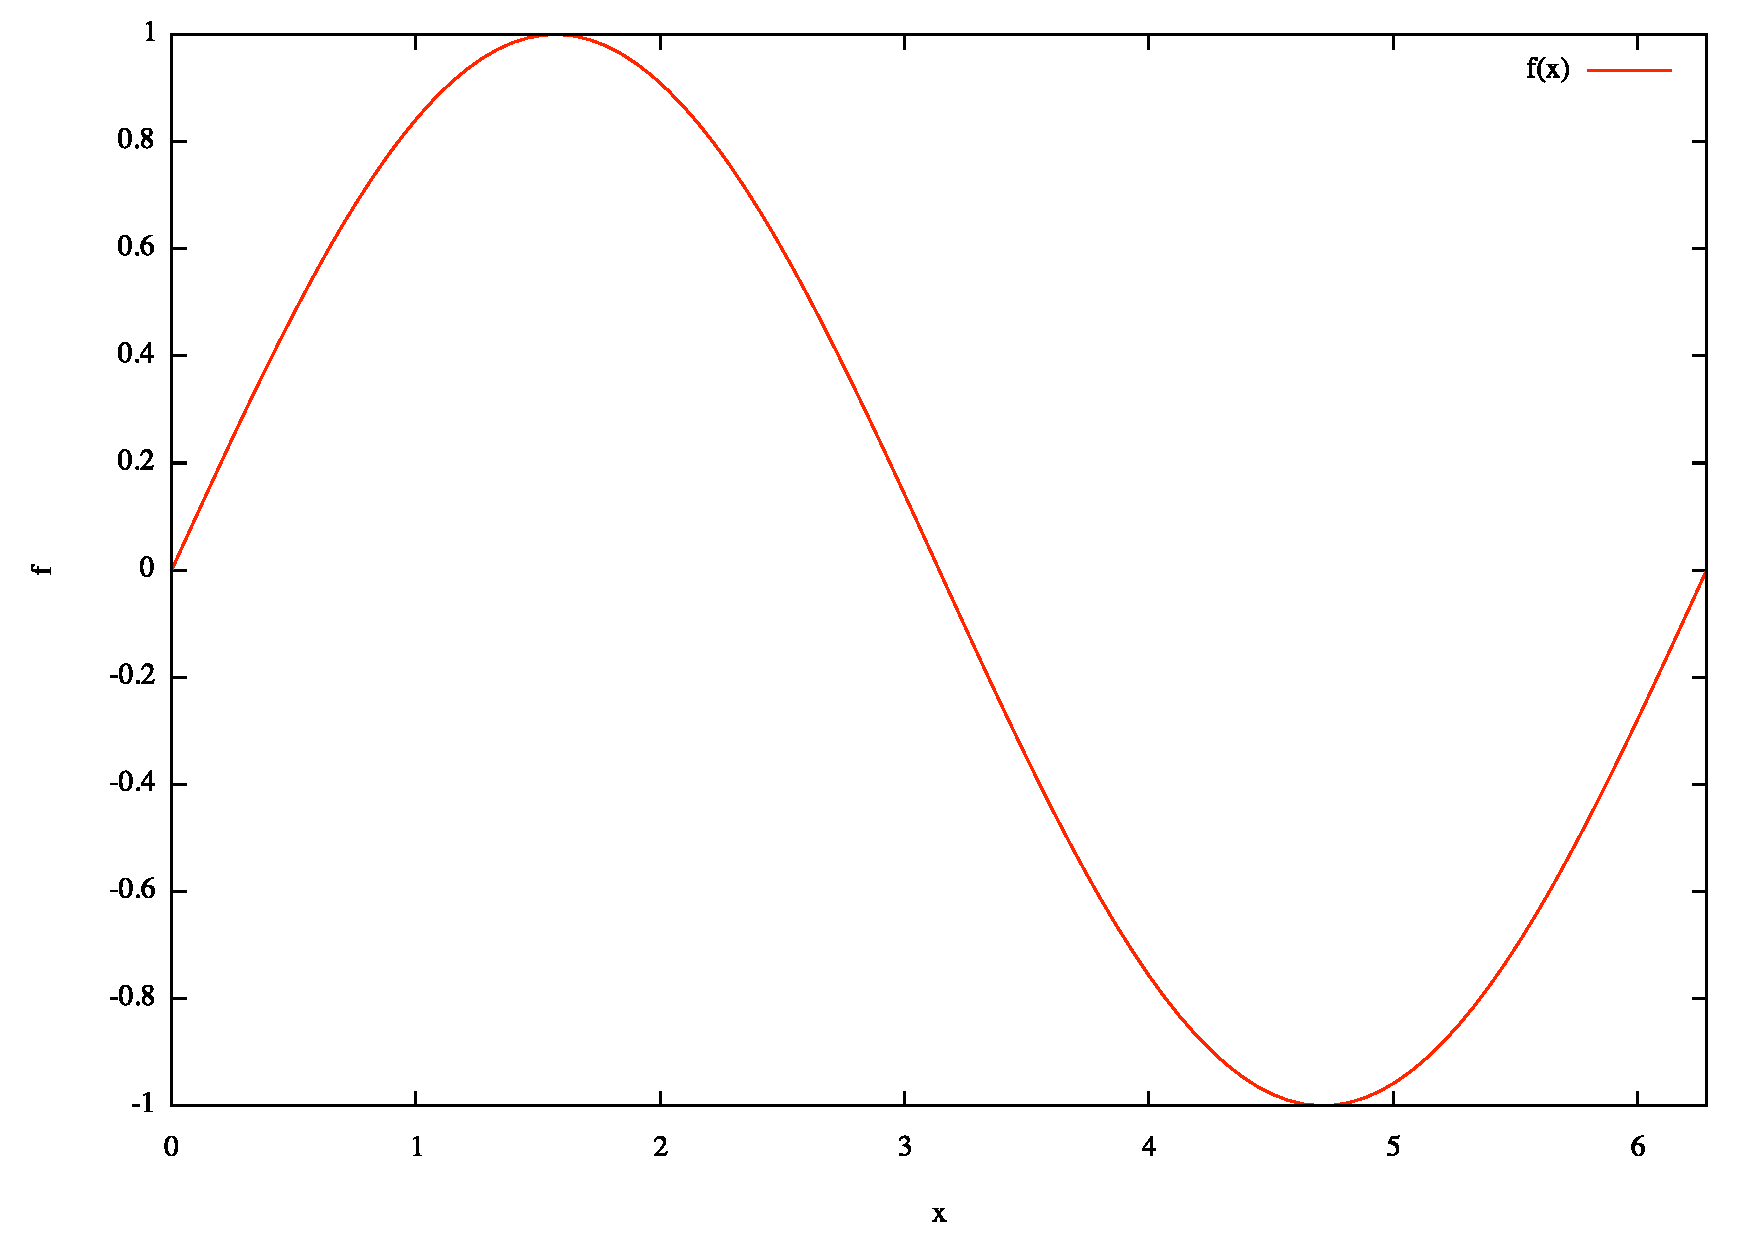
\includegraphics[width=.99\linewidth, height=.3\linewidth]{figure1.pdf}
\caption
{
\textbf{Kernels obtained in the self-supervised learning algorithm}: (a) 
\label{fig:fig1}
}
\end{figure}

\paragraph*{Hebbian Learning and the role of homeaostasis}
% we apply it to the N-MNIST dataset : prtesentation of this dataset
Blah blahblah blah blah blah. Blah blahblah blah blah blah Blah blahblah blah blah blah.
Blah blahblah blah blah blah. Blah blahblah blah blah blah Blah blahblah blah blah blah.
Blah blahblah blah blah blah. Blah blahblah blah blah blah Blah blahblah blah blah blah.
Blah blahblah blah blah blah. Blah blahblah blah blah blah Blah blahblah blah blah blah.
Blah blahblah blah blah blah. Blah blahblah blah blah blah Blah blahblah blah blah blah.
Blah blahblah blah blah blah. Blah blahblah blah blah blah Blah blahblah blah blah blah.

% we perform self-supervised learning as in Lagorce and obtain filters see Fig1 a
Blah blahblah blah blah blah. Blah blahblah blah blah blah Blah blahblah blah blah blah.
Blah blahblah blah blah blah. Blah blahblah blah blah blah Blah blahblah blah blah blah.
Blah blahblah blah blah blah. Blah blahblah blah blah blah Blah blahblah blah blah blah.
Blah blahblah blah blah blah. Blah blahblah blah blah blah Blah blahblah blah blah blah.
Blah blahblah blah blah blah. Blah blahblah blah blah blah Blah blahblah blah blah blah.
Blah blahblah blah blah blah. Blah blahblah blah blah blah Blah blahblah blah blah blah.

% there is an imbablance, we add homeostasis and obtain filters see Fig1 b
Blah blahblah blah blah blah. Blah blahblah blah blah blah Blah blahblah blah blah blah.
Blah blahblah blah blah blah. Blah blahblah blah blah blah Blah blahblah blah blah blah.
Blah blahblah blah blah blah. Blah blahblah blah blah blah Blah blahblah blah blah blah.
Blah blahblah blah blah blah. Blah blahblah blah blah blah Blah blahblah blah blah blah.
Blah blahblah blah blah blah. Blah blahblah blah blah blah Blah blahblah blah blah blah.
Blah blahblah blah blah blah. Blah blahblah blah blah blah Blah blahblah blah blah blah.


\paragraph*{Classifying using spikes}
% HOTS uses histograms : for N-MNIST it performs quite poorly
Blah blahblah blah blah blah. Blah blahblah blah blah blah Blah blahblah blah blah blah.
Blah blahblah blah blah blah. Blah blahblah blah blah blah Blah blahblah blah blah blah.
Blah blahblah blah blah blah. Blah blahblah blah blah blah Blah blahblah blah blah blah.
Blah blahblah blah blah blah. Blah blahblah blah blah blah Blah blahblah blah blah blah.
Blah blahblah blah blah blah. Blah blahblah blah blah blah Blah blahblah blah blah blah.
Blah blahblah blah blah blah. Blah blahblah blah blah blah Blah blahblah blah blah blah.


% Introduction 
Blah blahblah blah blah blah. Blah blahblah blah blah blah Blah blahblah blah blah blah.
Blah blahblah blah blah blah. Blah blahblah blah blah blah Blah blahblah blah blah blah.
Blah blahblah blah blah blah. Blah blahblah blah blah blah Blah blahblah blah blah blah.
Blah blahblah blah blah blah. Blah blahblah blah blah blah Blah blahblah blah blah blah.
Blah blahblah blah blah blah. Blah blahblah blah blah blah Blah blahblah blah blah blah.
Blah blahblah blah blah blah. Blah blahblah blah blah blah Blah blahblah blah blah blah.


\begin{figure}[!ht]%[!ht][!b]%
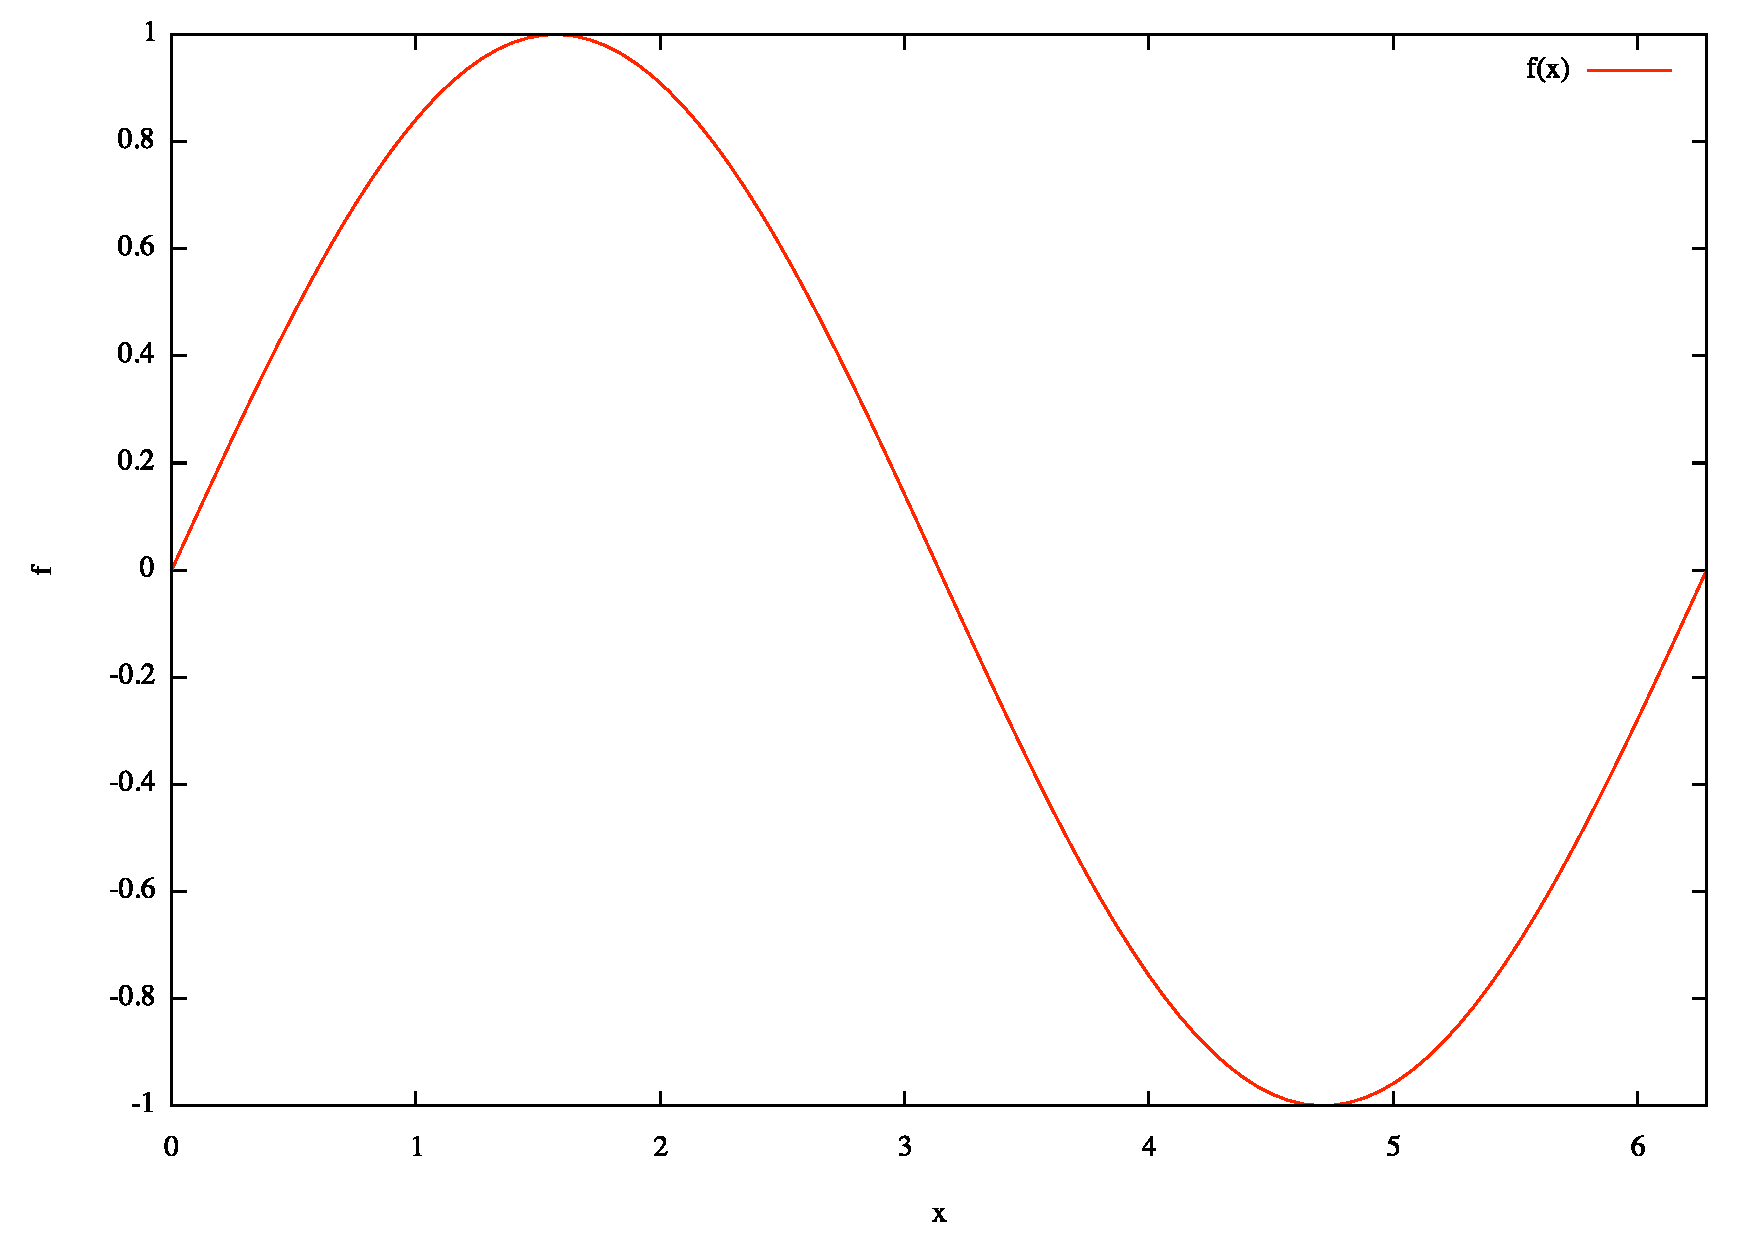
\includegraphics[width=.99\linewidth, height=.3\linewidth]{figure1.pdf}
\caption
{
\textbf{Temporal dynamics of the dynamics}: The final SNN can perform classification on an event-by-event basis. 
\label{fig:fig2}
}
\end{figure}



\vfil

%%%-----------------------------------------------------------------
%{\bf Acknowledgments}\\
%We thank T. Colleague for helpful discussions.
%This work was supported by NIH grant DC999999.

%%%-----------------------------------------------------------------
\printbibliography

\end{document}
